\chapter{A Terminological Classification}
\label{chap:apdxphysio}

In this chapter, we give the general outline how we have classified the touch technologies to isolate bilateral teleoperation which is 
our main focus. Moreover, we give some specific details about the human body for a quick reference.


\section{The Adopted Terminology}

The somatosensory system involves complicated chemical and mechanical components and there are different layers of sensory mechanisms 
that contribute to the overall perception. Hence, it is not always directly possible to use a reduction argument that simplifies the 
involved processes. In fact, depending on the type of sensation, different layers of these mechanisms are excited.

The main two branches of technology relating to the touch perception are the tactile and kinesthetic feedback (as we define below). The 
terminology is yet to reach a steady-state standard, however, what follows below seems plausible considering the variations and nuances found 
in the literature. Since there is no fixed definition for such perception we would use a rough  classification based on the magnitude-%
frequency content of the motion\footnote{In the sense of Fourier analysis}. We have to emphasize that this classification is completely 
conceptual and only serves to exclude the parts that are not studied in this thesis. Therefore, we refer the reader to the authoritative 
resources of the involved physiology, e.g., \cite{kandel}. We start with a somewhat detailed sensory classification to support our choice 
of amplitude-frequency based grouping.

Typically, the touch perception is also classified into these two groups; tactile feedback and kinesthetic (proprioceptive) feedback, 
hence the naming of the involved technologies. For practical purposes, one can use the analogy of parallel connected high-pass and low-pass 
filters to indicate the frequency band of interest respectively. For our control-oriented context, let us define a few key concepts with 
an engineering point of view. 

In physiology, the sensors on the skin which take different physical measurements are called \emph{receptors} and prefixed with their 
area of specialization such as \emph{thermoreceptors, mechanoreceptors, nocioreceptors} (pain) etc. The signals that trigger an action on 
these receptors are denoted as the \emph{stimuli}. In case of a stimulus, these receptors, through some chemical processes, exhibit a 
series of \emph{action potentials} or electrical discharge pulses i.e. a \emph{spike train}. In the engineering terminology, this can be 
modeled as a nonuniform Dirac comb with varying frequency as a function of the stimuli intensity or a digital frequency modulation (FM) 
signal. The frequency increases with the stimulus intensity. Furthermore, at the input side of this sensor there is a dead-zone 
nonlinearity hence the stimuli should exceed a particular threshold to trigger a receptor firing.

There is also another process, called \emph{neural} or \emph{sensorial adaptation} which quantifies the frequency decay of firing under constant 
stimulus. We can see the tangible effect of this process frequently e.g., our nose looses the sensitivity to a powerful smell if exposed 
to it for some time or we stop noticing the touch of glasses on the face or the ring on the finger. Some sensors have a slow decay 
rate whereas others decay in a matter of seconds. The slow sensors often called the \emph{slowly adapting (SA)} and others are called \emph
{fast adapting (FA)} or \emph{rapidly adapting} type \cite{burdea}.


As shown in \Cref{tab:mechano}, and also surveyed in \cite{kontarinis}, there are four main types of mechanisms that are utilized for the 
force and texture sensing with varying operating conditions and spatial authority. Although all contribute to the high frequency stimulus 
perception with varying levels, slowly adapting receptors are mainly tuned to detect the low frequency information range (up to \SI{30}{
\hertz}). The fast adapting Meissner(FAI) and Pacinian(FAII) Corpuscles can be excited in the frequency range of \SIrange{10}{60}{\hertz} 
and $\SIrange{60}{1000}{\hertz}$ respectively. Thus, small-area receptors (Type I) are excited with the rate of skin deformation whereas 
relatively large-area receptors (Type II) are with the acceleration of the skin. Moreover, FAI units are located closer to the skin 
surface, have high unit density with small surface area forming a grid of sensors. On the other hand, FAII units are located in the 
subcutaneous tissue and work as a single load cell with relatively large surface area. This allows experts to assume that FAI units are 
mainly responsible for spatial information about the skin deformation and FAII units are responsible for the high frequency information 
with response delays in the range of \SIrange{50}{500}{\milli\second} \cite{idareview}. Another interesting note in \cite{kontarinis} is 
that due to their single unit nature FAII units offers the possibility to provide high frequency information with a single vibration 
display, while for FAI units it is more appropriate to supply an array of haptic displays for lower frequency range.  

The SAI disk receptor has a small, localized receptive surface area as opposed to the SAII with a large field with a decaying sensitivity 
from center to the edges. Individual Ruffini endings are excited by stretch of the skin in specific directions. The majority of hand 
receptors consists of FAI units ($>40\%$), then SAI units cover almost a quarter which followed by SAII covering $19\%$ and FAII $13\%$. 



\newcolumntype{C}{>{\centering\arraybackslash}m{1.9cm}}%
\begin{table}%
\centering
\caption[Functional Features of Cutanous Mechanoreceptors]{Functional Features of Cutanous Mechanoreceptors (Adapted from \cite{idareview}
)}
{\tiny
\pgfplotstabletypeset[
column type=C,
every head row/.style={before row={\toprule},after row=\midrule,},
every last row/.style={after row=\bottomrule},
every even row/.style={before row={\rowcolor[gray]{0.9}}},
col sep=&,row sep=\\,
string type,
]{
Feature	                   &Meissner Corpuscles (FAI) &Pacinian Corpuscles (FAII) &Merkel's Disks (SAI) &Ruffini Endings (SAII)\\
Rate of adaptation         &Rapid                     &Rapid                      &Slow                 &Slow\\
Location                   &Superficial dermis        &Dermis and subcutaneous &Basal epidermis &Dermis and subcutaneous\\
Mean receptive area        &\SI{13}{\milli\metre\squared} &\SI{101}{\milli\metre\squared} &\SI{11}{\milli\metre\squared} &\SI{59}{
\milli\metre\squared}\\
Spatial resolution         &Poor&Very poor&Good&Fair\\
Sensory units              &43\%&13\%&25\%&19\%\\
Response frequency range   &\SIrange{10}{200}{\hertz}&\SIrange{70}{1000}{\hertz} &\SIrange{0.4}{100}{\hertz} &\SIrange{0.4}{100}{\hertz} \\
Min. threshold frequency   &\SI{40}{\hertz}&\SIrange{200}{250}{\hertz} &\SI{50}{\hertz}&\SI{50}{\hertz}\\
Sensitive to temperature   &No&Yes&Yes&At $>\SI{100}{\hertz}$\\
Spatial summation          &Yes&No&No&Unknown\\
Temporal summation         &Yes&No&No&Yes\\
Physical parameter sensed  &Skin curvature, velocity, local shape,flutter, slip &Vibration, slip, acceleration &Skin curvature, local 
shape, pressure&Skin stretch, local force\\
}
}% Closes the \tiny group
\label{tab:mechano}
\end{table}

\subsection{Weber ratio and Just-Noticeable-Difference(JND) }

The Weber ratio is defined as the ratio between the minimal stimulus intensity change in any physical quantity that triggers a change 
perception and the intensity of the stimulus. In case of a constant or static stimulus, the ratio is denoted with Just-Noticable-
Difference (JND). For engineering purposes, this derived unit can be beneficial to design the frequency behavior of the haptic systems 
which exhibit a particular sensitivity pattern.


\subsection{Tactile Feedback}

Tactile feedback, in general, is utilized to distinguish fine details such as shape, curvature, vibration, acceleration, and texture 
perception. Hence, the high-frequency content of the touch information is indispensable to transmit such information. Since the amplitude 
of the motion at these frequencies are quite small, the palm and finger tissues act as a low-pass filter and avoid such information to 
penetrate into the skin. Thus, only a limited part of the sensors have access to this information.

A striking example to the mind-boggling quality of feedback is the Braille system used by visually impaired or disabled individuals (\Cref
{fig:braille}). The average reading speed with Braille system is about 125-150 words per minute (\cite{americanblind}) in contrast with 
200-250 words per minute by eyesight. 

\begin{figure}%
\centering
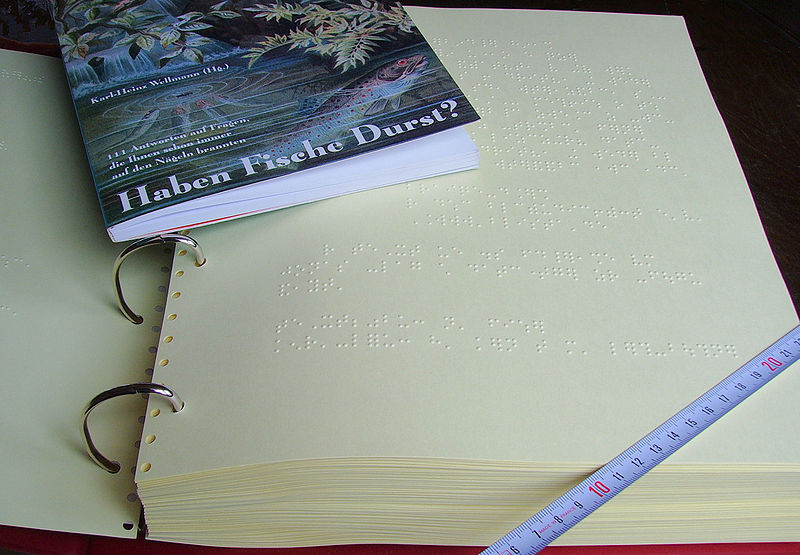
\includegraphics[width=0.8\columnwidth]{\impath/intro/braille.jpg}%
\caption[The length comparison of the same content in the form of Braille and 
regular text]{A comparative case for the spatial resolution: The volume of the same 
content in the form of Braille and regular text (Karl-Heinz Wellmann, 
\href{http://de.wikipedia.org/wiki/Brailleschrift}{[Wikipedia:Brailleschrift]})}%
\label{fig:braille}%
\end{figure}

Most of today's technological devices utilize this modality to send and receive information. Many mobile phone applications and a few 
gaming consoles such as Nintendo Wii\raisebox{0.5ex}{\scriptsize\texttrademark}, Sony Playstation\raisebox{0.5ex}{
\scriptsize\texttrademark} etc., utilize short vibrational patterns to alert the user that some action has been performed e.g. the user 
hovers over a hot spot on the screen or some moving object hits an obstacle etc. 

The tactile technology is, thus, concerned with the vibrational pattern and high-frequency sweep of stimuli. Communication via small 
vibrational or textural subtleties allows the tactile technology to focus on the low-stroke, high-bandwidth haptic displays. The required 
low-stroke action is often generated by a small and agile electrical motor with a load eccentricity with respect to the rotor shaft axis. 
The angular velocity of the motor then defines the frequency of the vibration. Since the involved mechanisms on the human limbs and hands 
are rapidly adapting, the bus speed in this modality can be very high compared to the kinesthetic feedback in which the human should 
track and pick out patterns from relatively slow and large-amplitude motion profiles via measuring muscle stretch amount and various 
other quantities. 


\subsection{Kinesthetic (Proprioceptive) Feedback}
Proprioception\footnote{We will not go into the nuances between kinesthetic and proprioceptive feedback} (\emph{Proprius}+\emph{perceptio}
: the act of gathering/perceiving of own) is the ability to sense the limb configurations and motion without using a visual aid (cf. 
vestibular feedback which is to used to sense the balance and the spatial body orientation). Kinesthetic feedback, together with limited 
force sensing abilities of muscles and tendons and relatively small interference of tactile feedback system, is \enquote{vital} to have 
control of our own body. It's a futile attempt to describe the importance of this often overlooked perception (or hidden sense) other 
than referring to the 1998 BBC \emph{Horizon} documentary \enquote{\emph{The man who lost his body}} and the paper \cite{waterman} about 
Ian Waterman. He is the only person known to date who can cope with the loss of proprioceptive feedback while still being able to stand 
up, walk, maintain posture etc. without any artificial support. Unfortunately, he is completely dependent on his visual feedback as he 
tirelessly computes trajectories of his body parts on-the-fly to compensate for the loss of kinesthetic feedback even when gesturing with 
hands. 

Thus, whether we are aware of it or not, proprioception is indispensable for us to survey the environment. The force on our limbs, our 
body configuration at that instance, and our body motion are sensed via sensors in the joints, muscle tendons and muscles themselves. Unlike 
the tactile feedback characteristics given previously, the compliance, the distribution of pressure and and the shape information is 
measured in a relatively coarse fashion. Hence, when combined with tactile feedback and the brain's internal comparison database, we use 
an unparalleled sophistication to actually perceive the environment without using any visual feedback, even if the object is foreign to us. 
In \cite{biggssrinivasan}, a convenient summary of the properties is presented. Distilling even further for a general picture about the 
proprioception, we provide the following quick facts. 

The compression or stretch of the receptors covered previously changes the amplitude of the impulse of the action potential which, in turn, 
used as the position information. Similarly the frequency of these firings are interpreted as the velocity information. For the limb 
position and motion, the bandwidth of the kinesthetic sensing is around \SIrange{20}{30}{\hertz} with varying accuracy in terms of JND 
around \SIrange{0.8}{2.5}{\degree}. Moreover, the control bandwidth is reported to be task-dependent: \SIrange{1}{2}{\hertz} for 
unexpected signals; \SIrange{2}{5}{\hertz} for periodic signals, \SI[parse-numbers=false]{<5}{\hertz} for generated or learned 
trajectories and finally about \SI{10}{\hertz} for reflex actions. 

Regarding the force sensing, it has been experimentally demostrated that pressure JND decreases as the pressure area increases; e.g., the
overall average JND drops to $3.7\%$ with a contact area of \SI{20.27}{\centi\meter\squared} from $15.6\%$ with a contact area of \SI{1.27
}{\centi\meter\squared}. 

The kinesthetic technology can be used in conjunction with tactile technology to provide a full manipulative immersion. Moreover, in the 
case of \emph{exoskeletons}, it can be the essential ingredient to protocol between the environment and the human body. Especially, 
rehabilitation patients can benefit from such technologies via combining the visual and the kinesthetic feedback to amplify the disabled 
or impaired control action of the problematic limb. Thus, kinesthetic technology is mainly involved as low-frequency based manipulative 
or explorative motion tasks. Considering the current hardware limitations, many tasks depend primarily and rather primitively on kinesthetic 
cues for bilateral teleoperation and virtual reality applications.


\subsection{Teleoperation}
Teleoperation is the general name for providing human actions to a different media that is not accessible (or only in a costly way) to 
direct contact in a precise fashion. Microcomponent assembly, minimal invasive surgery (MIS), space station maintenance and construction, 
underwater exploration and construction are all typical application examples that the human either can not be present or physically 
interact with comfortably. The \emph{da Vinci}\raisebox{0.5ex}{\scriptsize\texttrademark} surgery robot from Intuitive Surgical Inc. is a 
well-known example of \emph{unilateral} human manipulation to achieve high precision tracking with surgical tools inside very tight 
incisions. 

However, as often motivated by the \emph{bilateral} teleoperation studies, the human operators, expecially the experienced ones, often 
lack the ability to employ their precise tactile and kinesthetic abilities to take decisions or to monitor their progress since they rely 
on vision feedback from the cameras exclusively. In some particular practices, surgeons might resort to inserting their fingers inside 
the incision to feel the relevant tissue stiffness difference to get a better spatial understanding when the view is contaminated with 
blood or other bodily fluids. In the case of an obstruction during an insertion of an instrument into the body, they might tend to 
correct the instrument based on their force feel at hand. Hence, the realism is diminished as opposed to the increased precision by the 
teleoperation methods. 

\subsection[Haptics]{(Computer) Haptics}
In general, haptics technology encompasses all the items that have been covered up to this point. However, it is also often used as a 
placeholder for the concept of creating artificial or virtual object perception with a force-feedback capable device. Computer haptics 
also have additional challenges such as rendering deformations in case of a soft object or realistic graphical presentation of object 
interaction in terms of collisions etc. In other words, not only the forces are important but the consequences of these force 
interactions need to be handled in a precise fashion. Conversely, computer haptics is free from the hardware limitations or the noisy 
measurements, as the objects and the physical laws that they should obey are computer generated. 


\subsection{Virtual Reality}

This term refers to a set of artificially generated immersion techniques that can rely on either a single or multiple modalities at once. 
The common applications consist of special googles that cover the human vision. By tracking the head movements and adjusting the scene 
that is projected onto the special headset, the user can immerse into the artificial environment. Combined with headphones and if possible 
with haptics, the experience can be substantially improved. Especially haptics can increase the immersion level much more compared to 
only visual+audio supplements since otherwise the realism can be destroyed quickly if the user tries to touch any object or surface while 
actually waving his hand. The persuasiveness of the scene depicted on the headset needs to be backed up with at least a slight 
kinesthetic feedback, if not tactile, since the loss of tactile feedback is relatively less important in an exploration task. 
